\documentclass[letterpaper]{article}
\usepackage{underscore}
\usepackage[left=2.0cm, right=2.0cm, top=1.0cm]{geometry}
\usepackage[utf8]{inputenc}
\usepackage{graphicx}
\usepackage{graphics}
\usepackage[spanish]{babel}
\usepackage{lipsum}
\usepackage{float}
\usepackage{subfigure}
\usepackage{csquotes}
\usepackage{color}
\usepackage{colortbl}
\usepackage{xcolor}

\title{EV\_1\_3\_circuitos\_de\_control\_de\_voltaje\_y\_corriente\_con\_tiristores}
\author{Ledesma Hernández Miguel Ángel \\ \&\& \\ Alcantar Días Joel Alejandro}
\date{28/10/2019}

\begin{document}
\begin{figure}[t]
    
\includegraphics[width=6cm]{img/logo.png}
\end{figure}
\vspace{2cm}
\maketitle
\vspace{12cm}
\begin{center}
   Universidad politécnica de la zona metropolitana de Guadalajara.\\
Sistemas electrónicos de interfaz.\\
4-A Mecatrónica.\\ 
\end{center}
\newpage

\begin{LARGE}
\textbf{Objetivo:}\\
\end{LARGE}

1.-Crear un sistema que regule el voltaje y corriente usando tiristores principalmente, demostrado por la intensidad de luz de un foco\\
2.- Simular reguladores de voltaje y corriente con tiristores mediante pulsos.

\begin{LARGE}
\textbf{Materiales:}\\
\end{LARGE}

\begin{table}[htbp]
\begin{tabular}{|l|l|}
\hline
{\color[HTML]{3166FF} \textbf{Equipo}} & {\color[HTML]{CB0000} \textbf{Componentes}} \\ \hline
Multímetro                             & Potenciometro 500K$\Omega$                  \\ \hline
Protoboard                             & Resistencias varias                         \\ \hline
Foco/clavija/switch                    & Cables/caimanes                             \\ \hline
                                       & Diac DB3                                    \\ \hline
                                       & Triac BT138                                 \\ \hline
                                       & Condensador cerámico                         \\ \hline
\end{tabular}
\end{table}

\begin{LARGE}
\textbf{Procedimiento:}\\
\end{LARGE}

%Super Proceso 
\begin{itemize}
    \item \textbf{1.- Se arma el circuito}
    \begin{itemize}
        \item Colocar el potenciometro cómo referencia para los demás componentes 
        \item De la pata media poner una resistencia de 10K$\Omega$ [café, negro,naranja] que irá a positivo
        \item Conectar el condensador cerámico a alguna de las patas restantes y este a su vez conectado al negativo
        \item Conectar Diac[DB3] a la pata seleccionada del potenciometro y el condensador cerámico 
        \item Conectar el otro extremo del DB3 a una resistencia de 100$\Omega$ [café, negro, café]
        \item Conectar el triac según su datasheet[en este caso la siguiente], la resistencia debe ser conectada al "gate" o "gatillo" del triac.
        \begin{figure}[htbp]
            \centering
            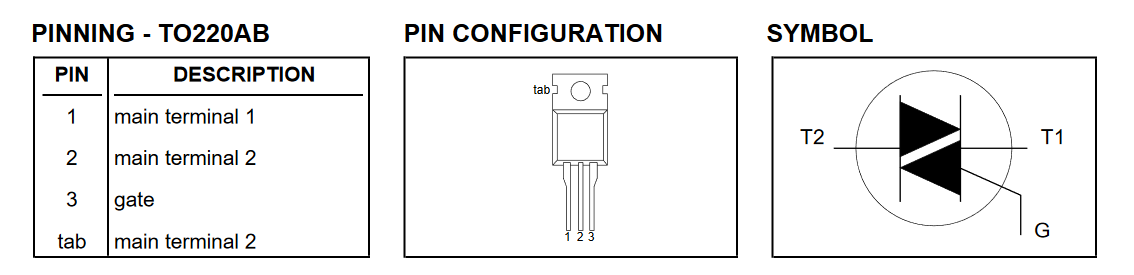
\includegraphics[width=15cm]{img/triacdatasheet.PNG}
            \caption{Datasheet Triac[BT138]}
            \label{fig:my_label}
        \end{figure}
        \item Conectar Terminal1[T1] de el triac a neutro
        \item Conectar Terminal2[T2] dos a fase 
        \item Identificar conexiones en el tomacorriente
            \begin{itemize}
                \item Poner multímetro para voltaje en alterna
                \item introducir una punta del multímetro en el tomacorriente
                \item tocar una tierra física con la otra punta (puede ser el tornillo que une la caja con la pared)
                Si el multimetro muestra lectura de al rededor de 120v, dependiendo del pais, se esta tomando la lectura de fase, si por el contrario el multimetro no muestra lectura, hay 0v, se esta tomando lectura de neutro.
            \end{itemize}
        \item Conectar nuestro circuito del socket, el foco en serie con fase y el triac como se muetra en la figura 2
        \newpage
        \begin{figure}[htbp]
            \centering
            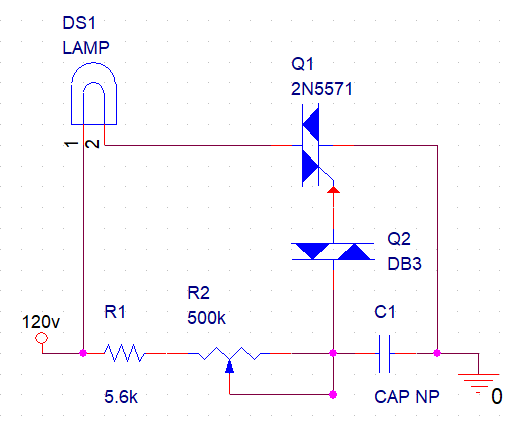
\includegraphics[scale=0.5]{img/arturo.png}
            \caption{Circuito regulador de intensidad}
            \label{fig:cirlamp}
        \end{figure}
        \item Probar que todo funcione correctametne
    \end{itemize}
    \item Una vez funcione como debe. Tomar las medidas de resistencia en el potenciometro de cada estado.\\
\end{itemize}
\textbf{Procesos de simulación}\\
\begin{large}
        \begin{enumerate}
            \item Se observa el esquema de la simulación a realizar.
            \item Se marca la opción para solo utilizar componentes que se puedan simular.\\
                  (En la practica se menciona que se debe realizar un modelo de tiristor pero si OrCAD ya lo incluye no es necesario).
            \item Seleccionar los componentes necesarios para la elaboración de la simulación.
            \item Colocarlos y seguir el esquema marcado en la practica.
            \item Simular colocando las puntas de la manera indicada.
            \item Corroborar que las gráficas sean similares a las presentadas en la practica.
        \end{enumerate}
    \end{large}
\begin{LARGE}
\textbf{Resultados:}\\
\end{LARGE}
\begin{large}
    Se consigue regular la intensidad del foco utilizando el potenciometro; mostrando 4 estados de intensidad lumínica: Apagado, intensidad 1, intensidad 2 y máxima potencia. Se analiza cómo funciona el triac en conjunto con el diac, para intencificar o reducir su fuerza lumínica.\\
    Ya con el potenciometro se facilito el poner resistencias al circuito y se pudo cambiar exitosamente al diseño original.\\
    \newpage
    \textbf{Simulaciones:}\\
    1.\\\\
    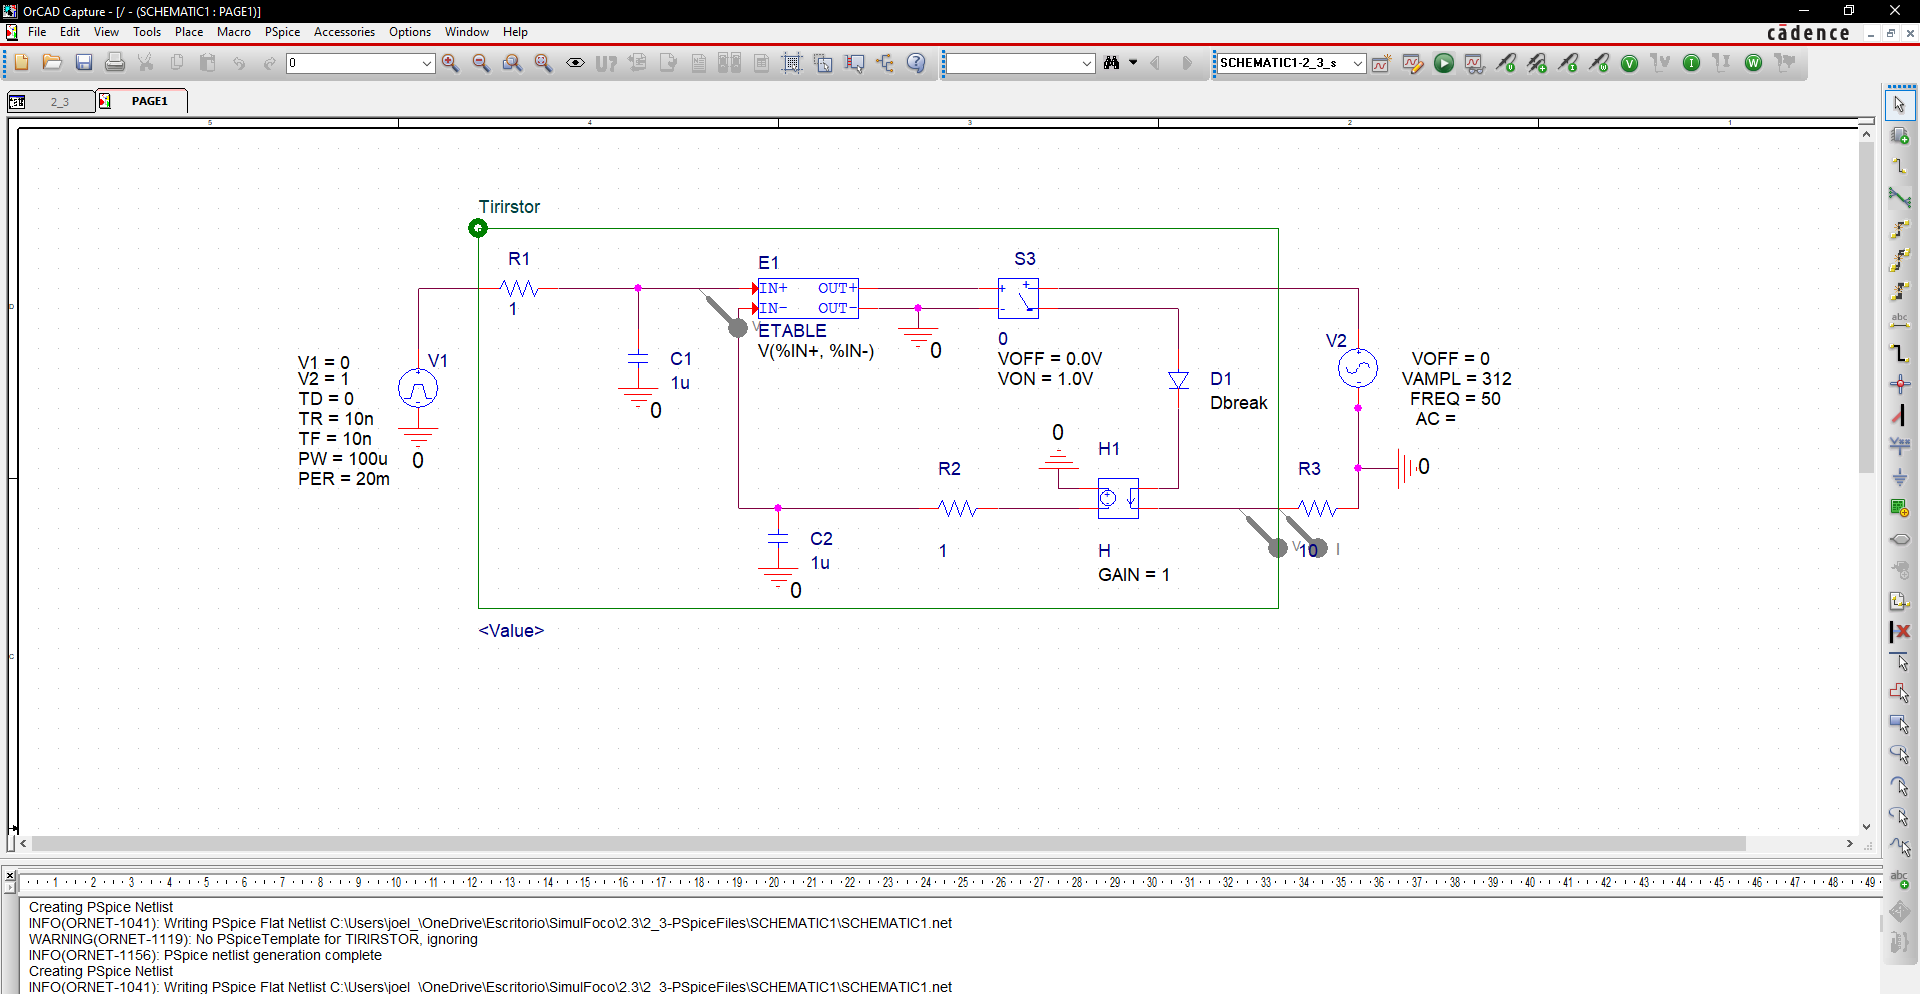
\includegraphics[width=13cm]{img/Sim/1.png}\\
    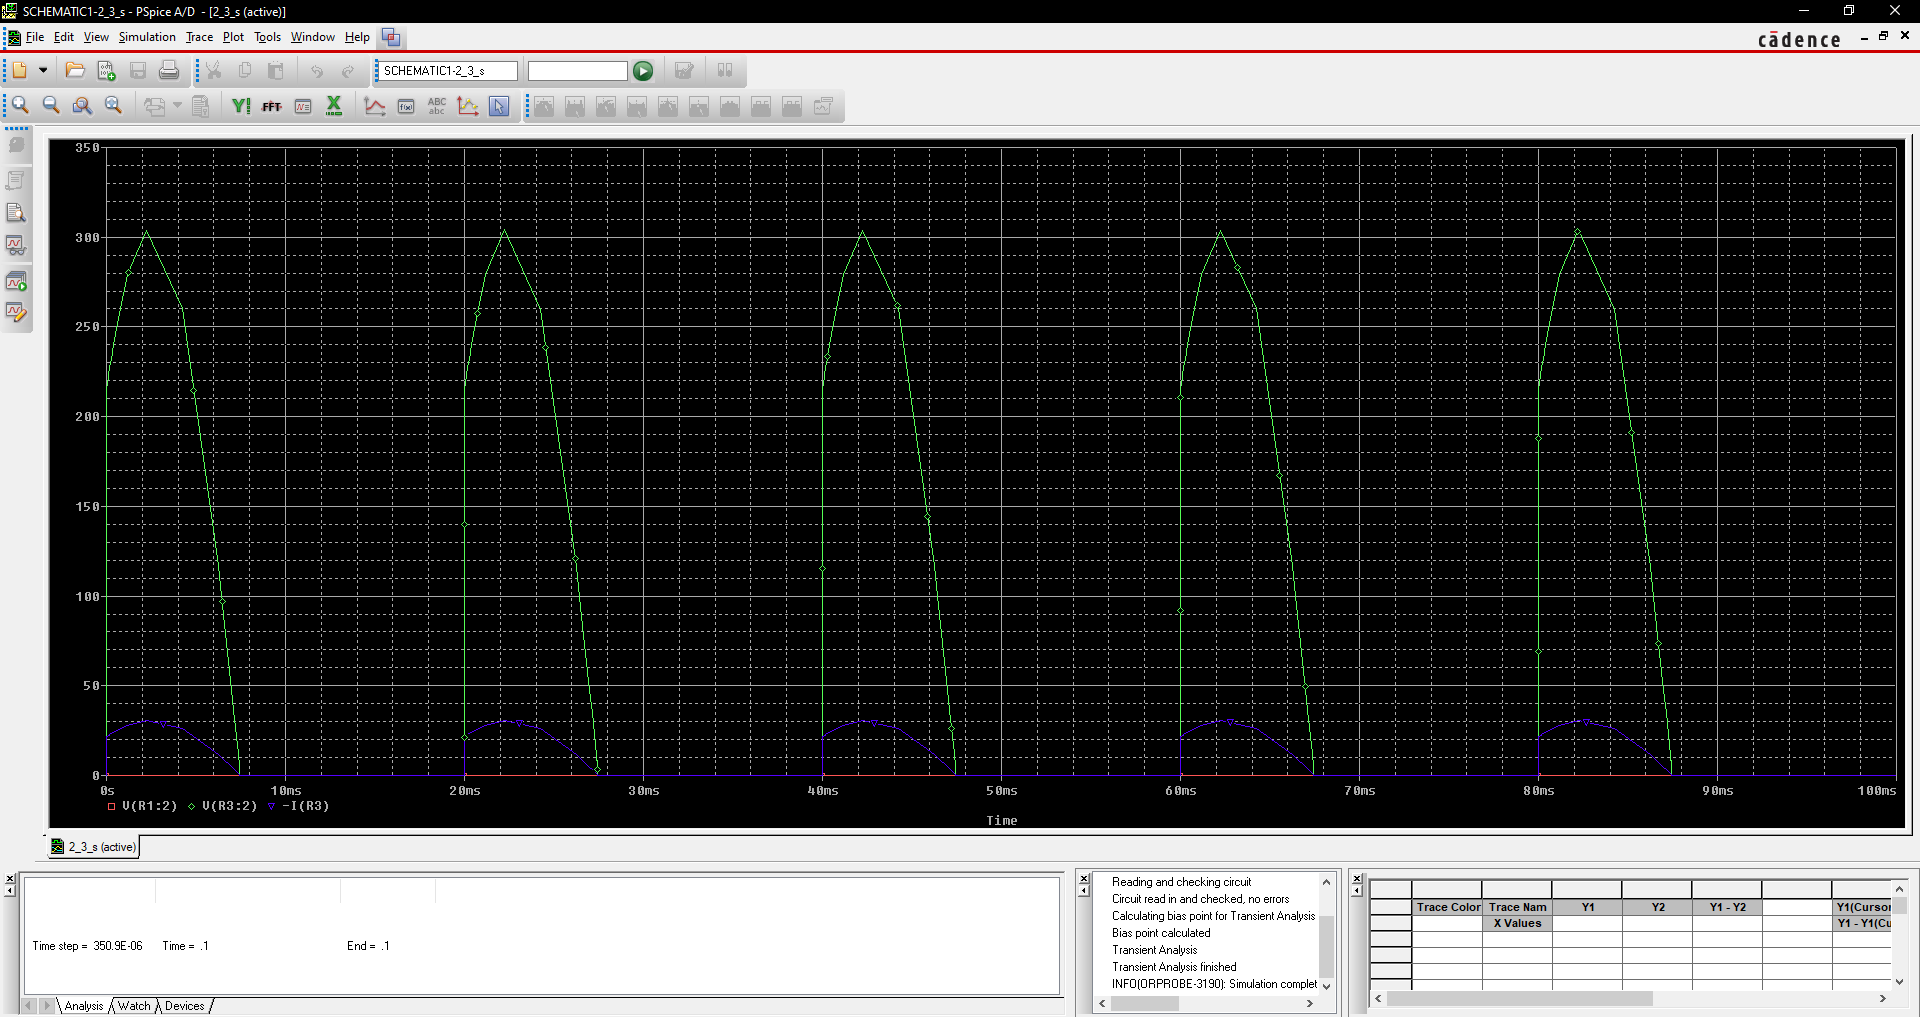
\includegraphics[width=13cm]{img/Sim/11.png}\\\\
    2.\\\\
    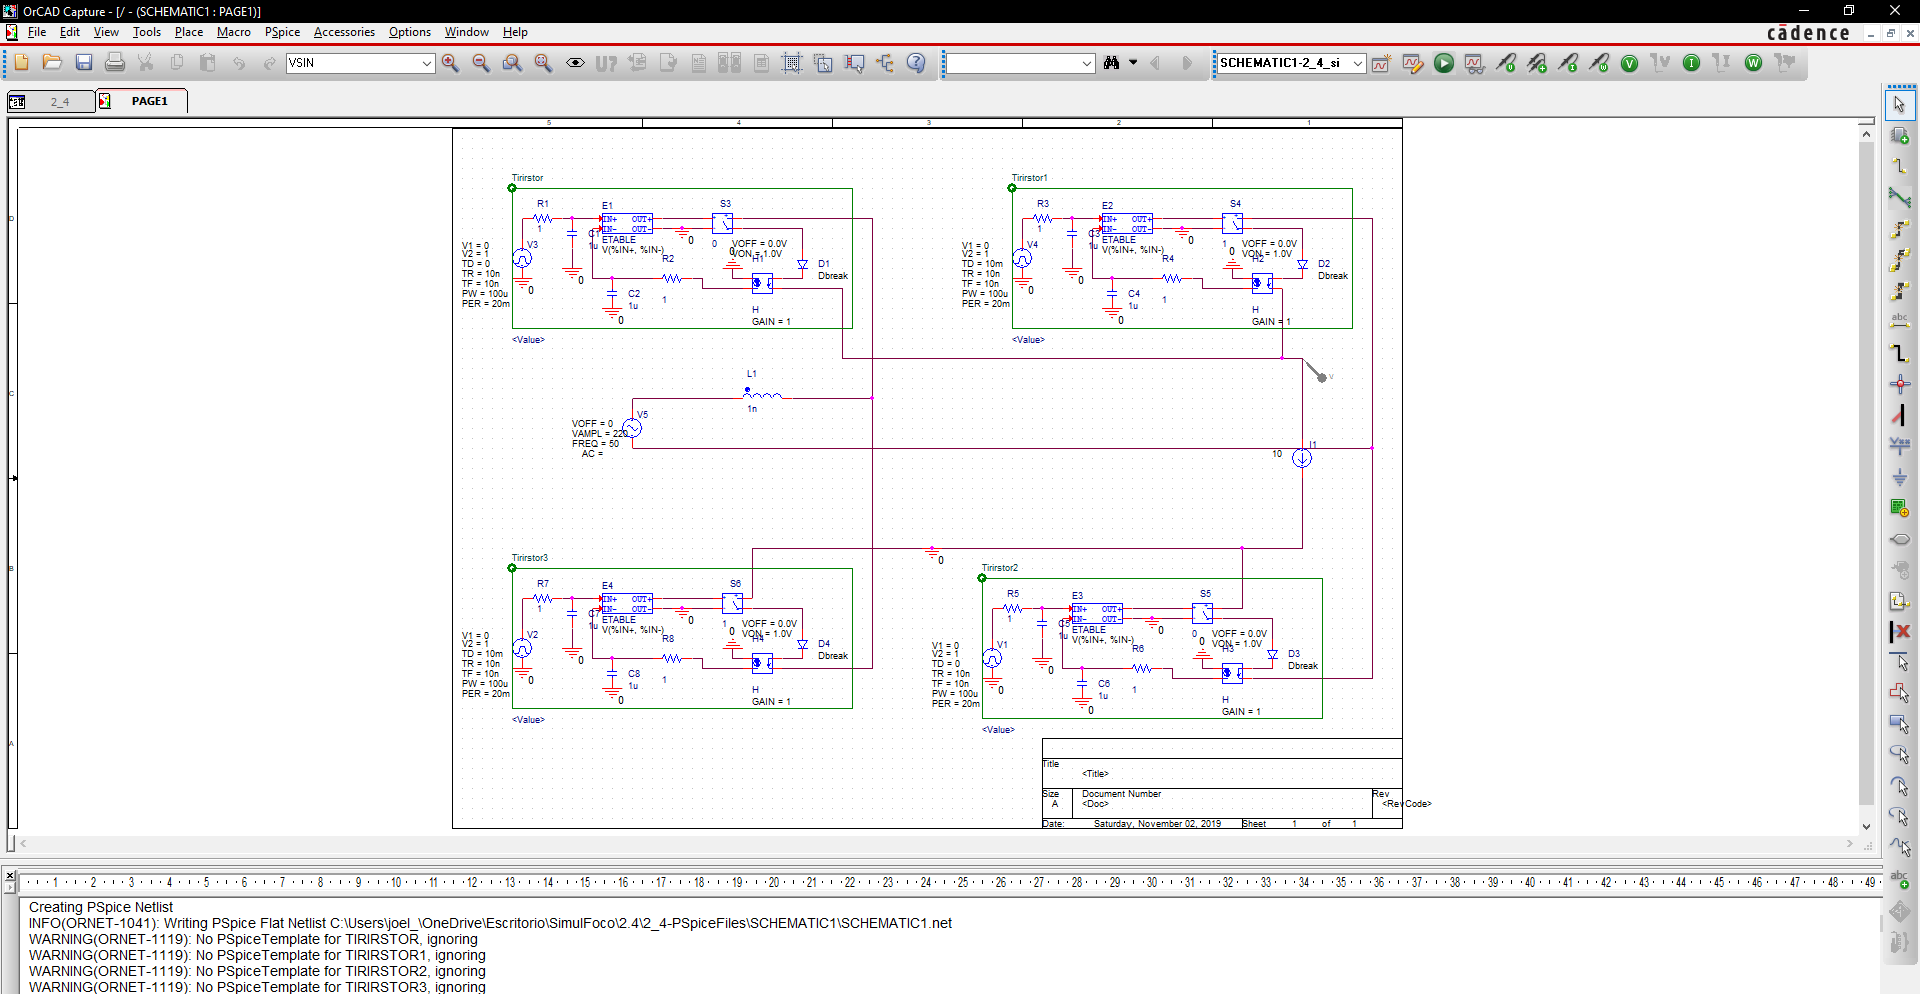
\includegraphics[width=13cm]{img/Sim/2.png}\\
    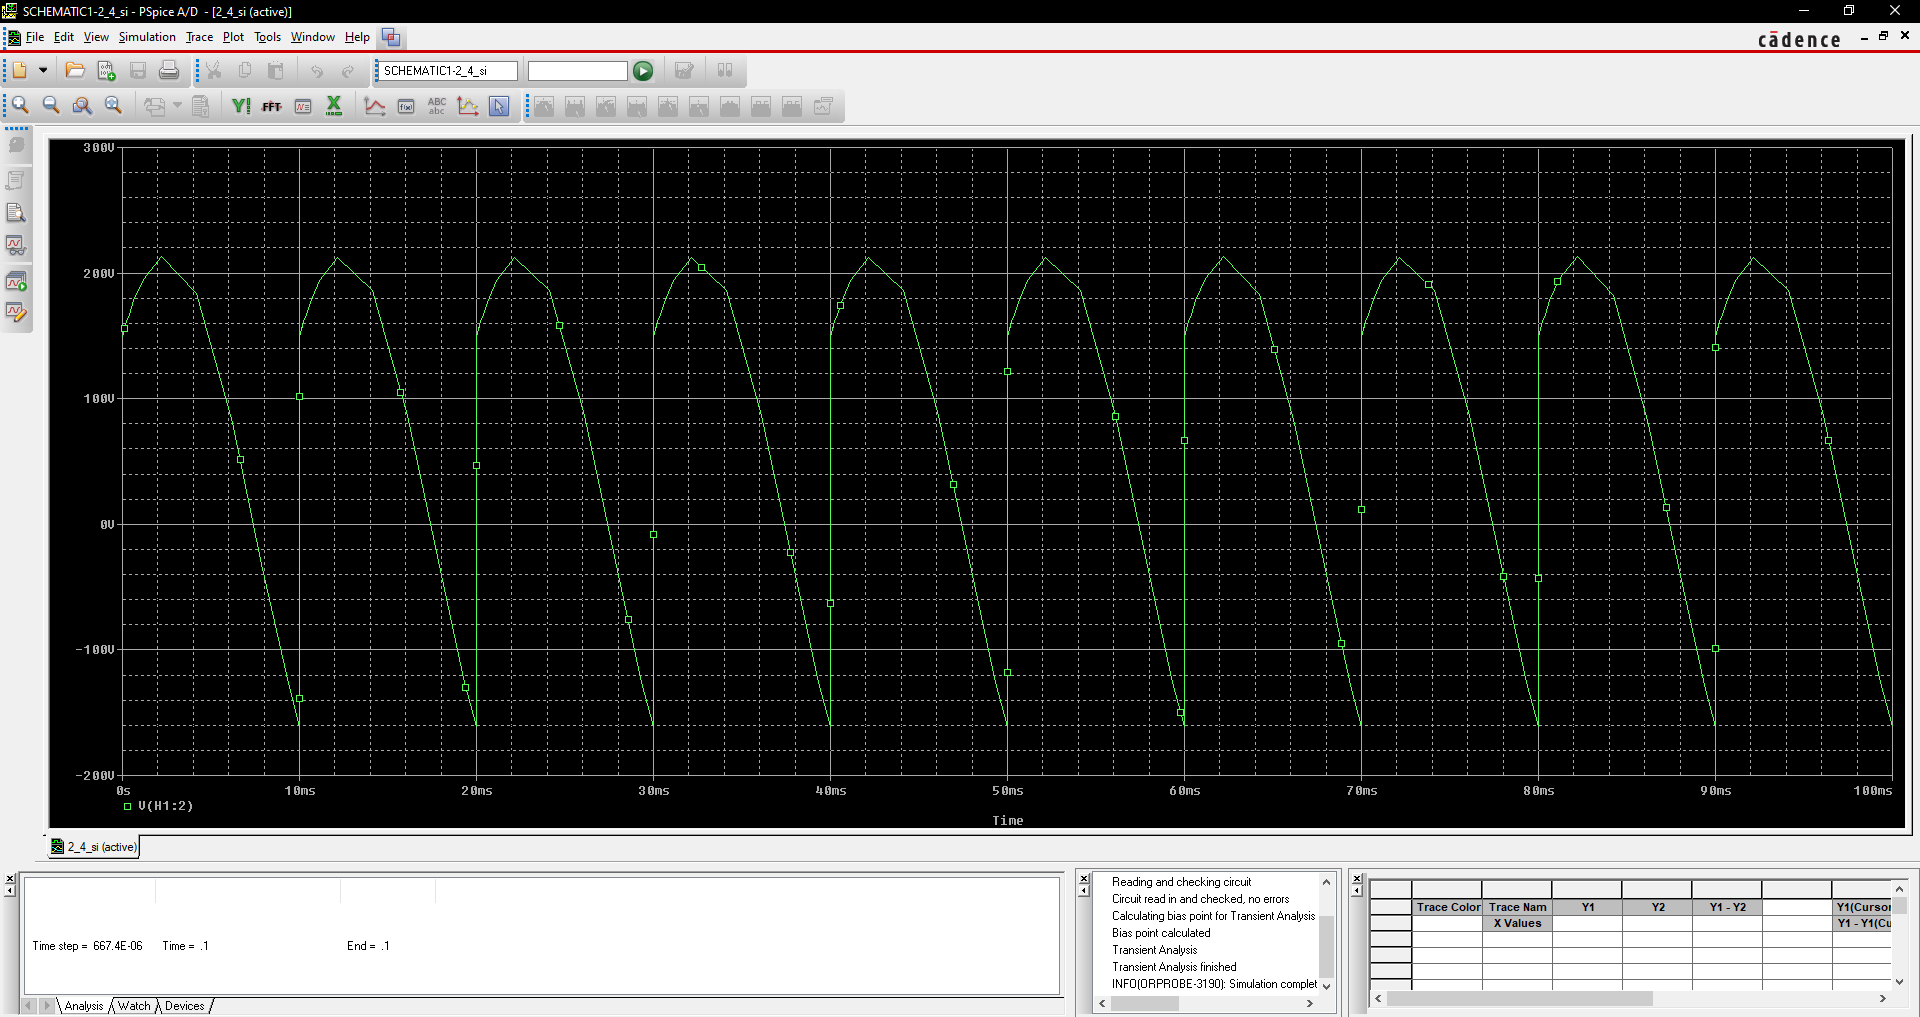
\includegraphics[width=13cm]{img/Sim/22.png}\\\\
    3.\\\\
    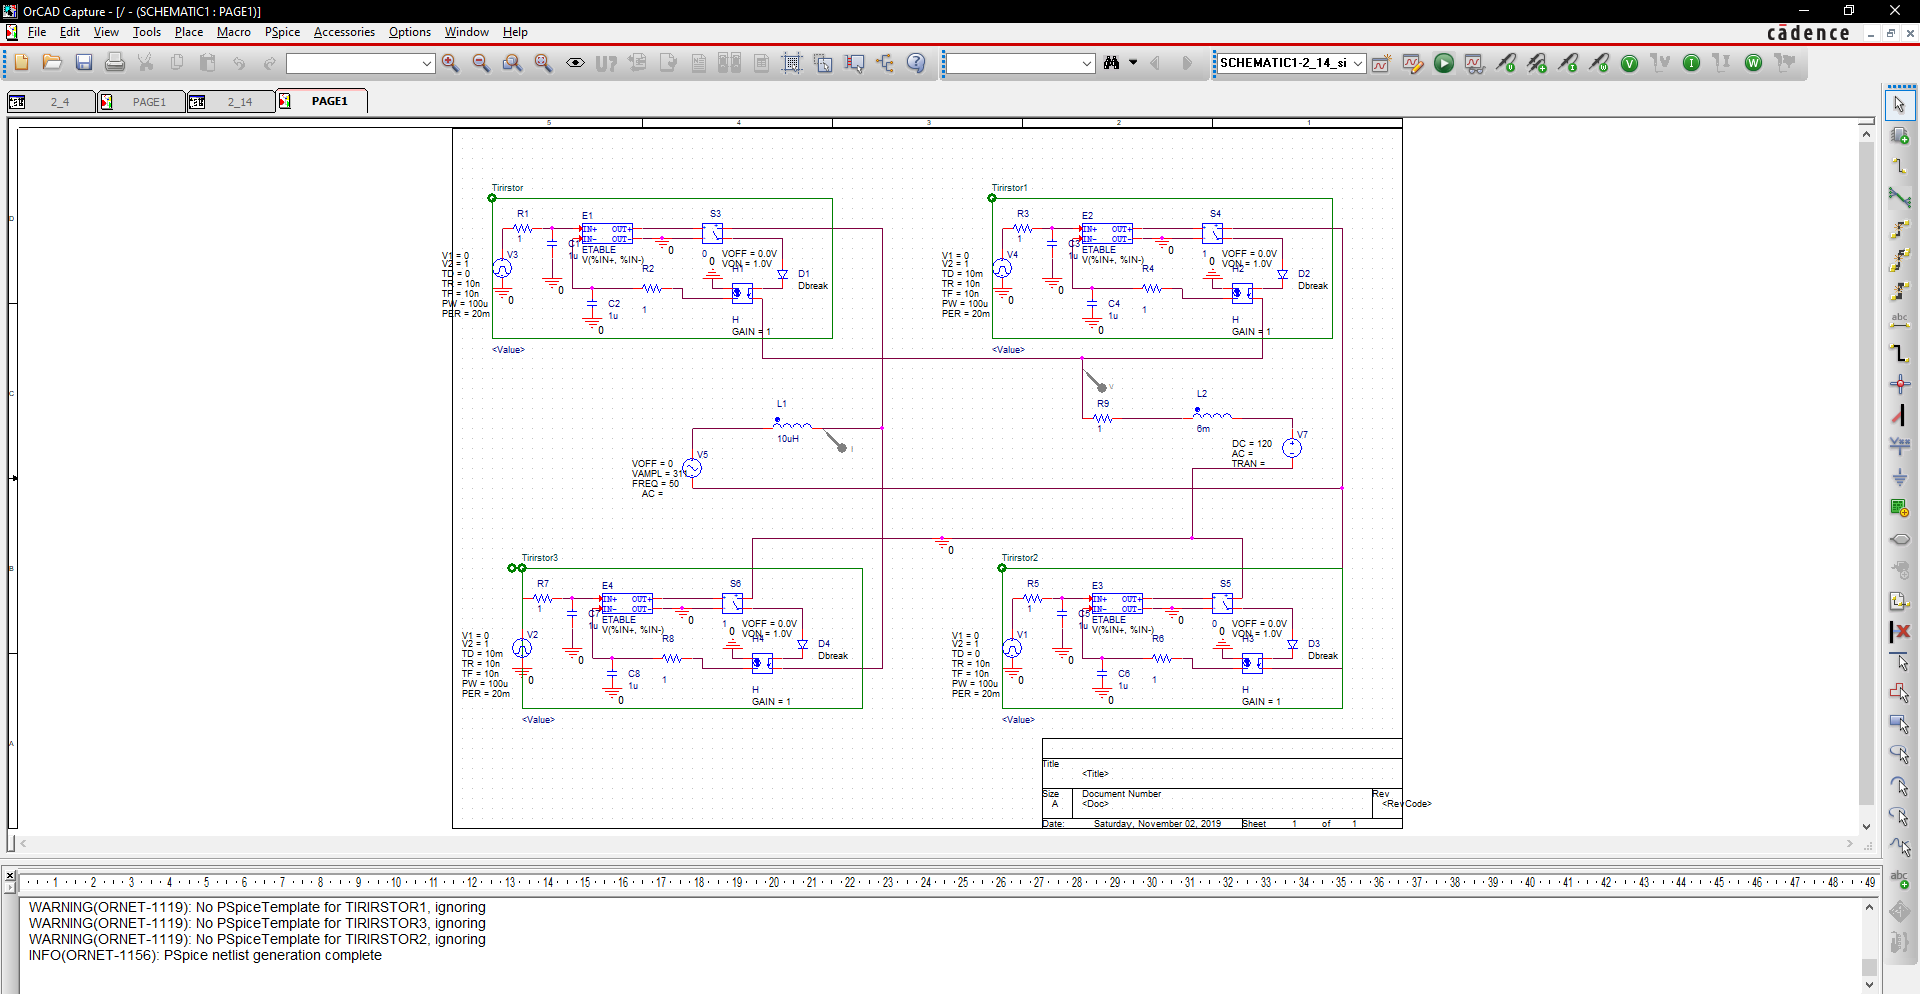
\includegraphics[width=13cm]{img/Sim/3.png}\\
    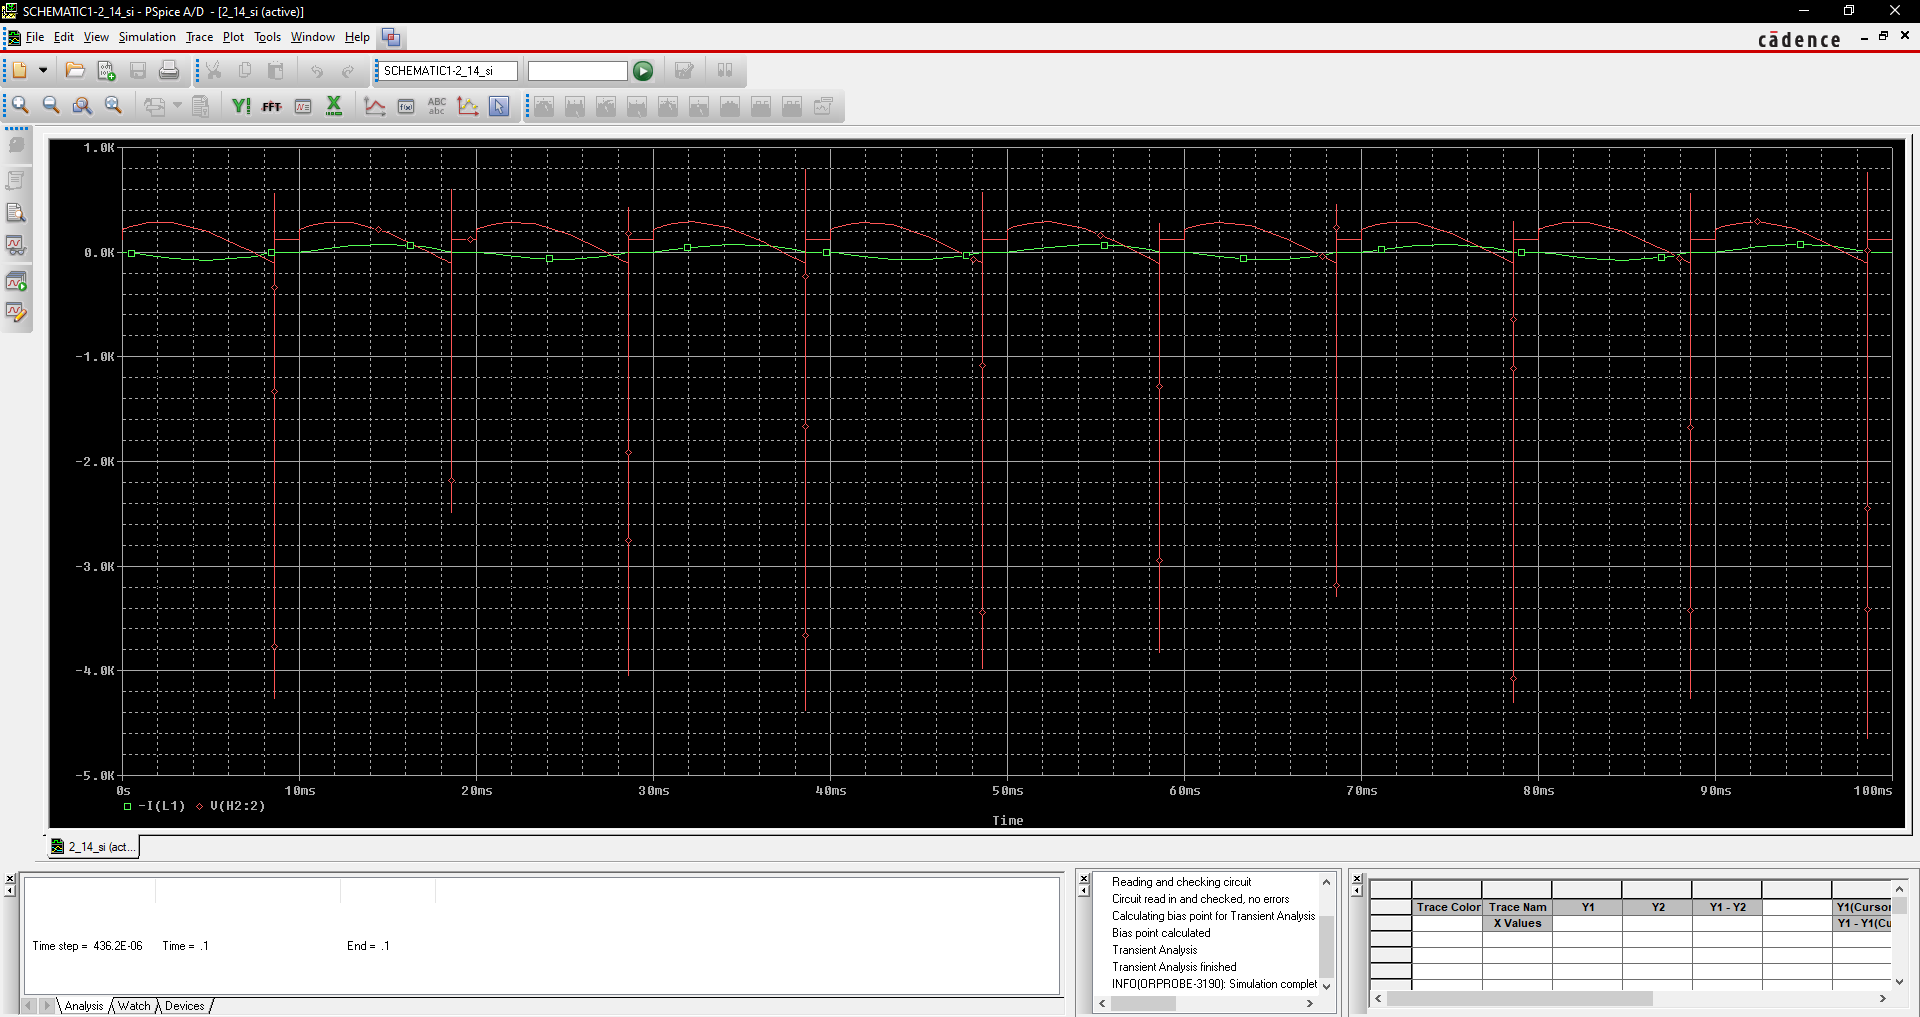
\includegraphics[width=13cm]{img/Sim/33.png}\\\\
    4.\\\\
    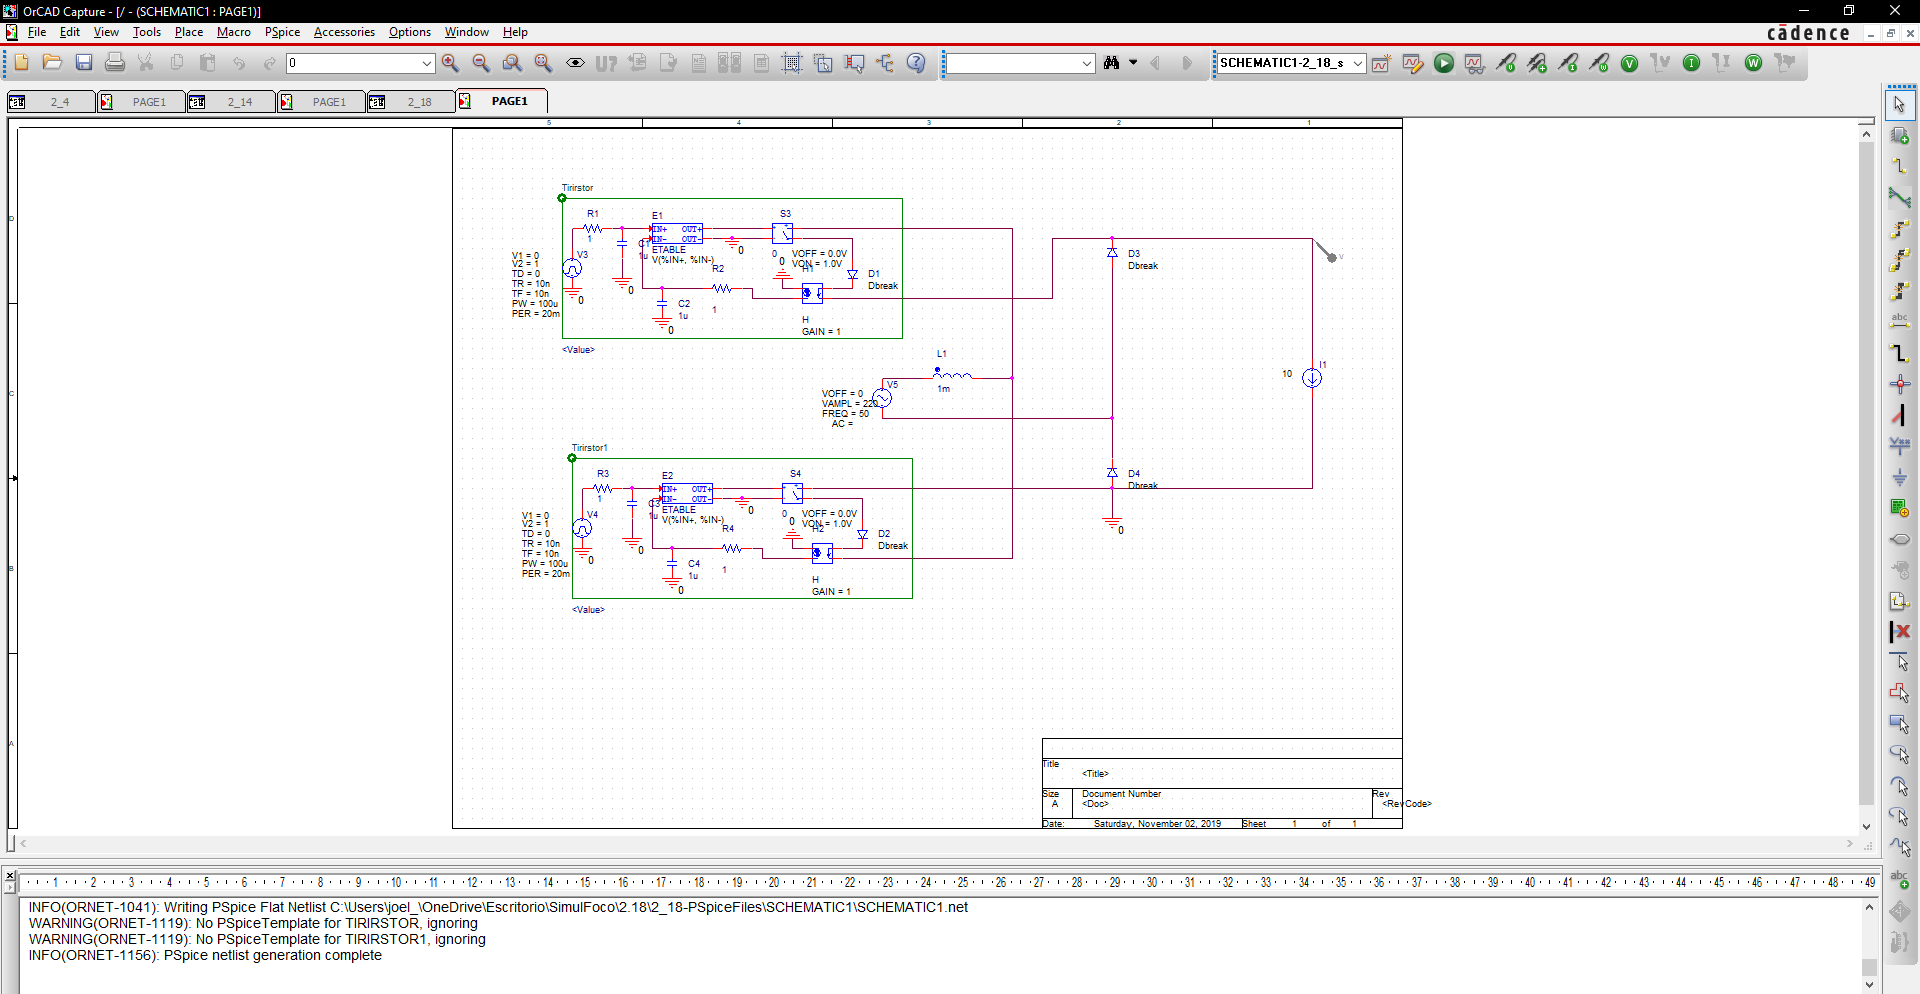
\includegraphics[width=13cm]{img/Sim/4.png}\\
    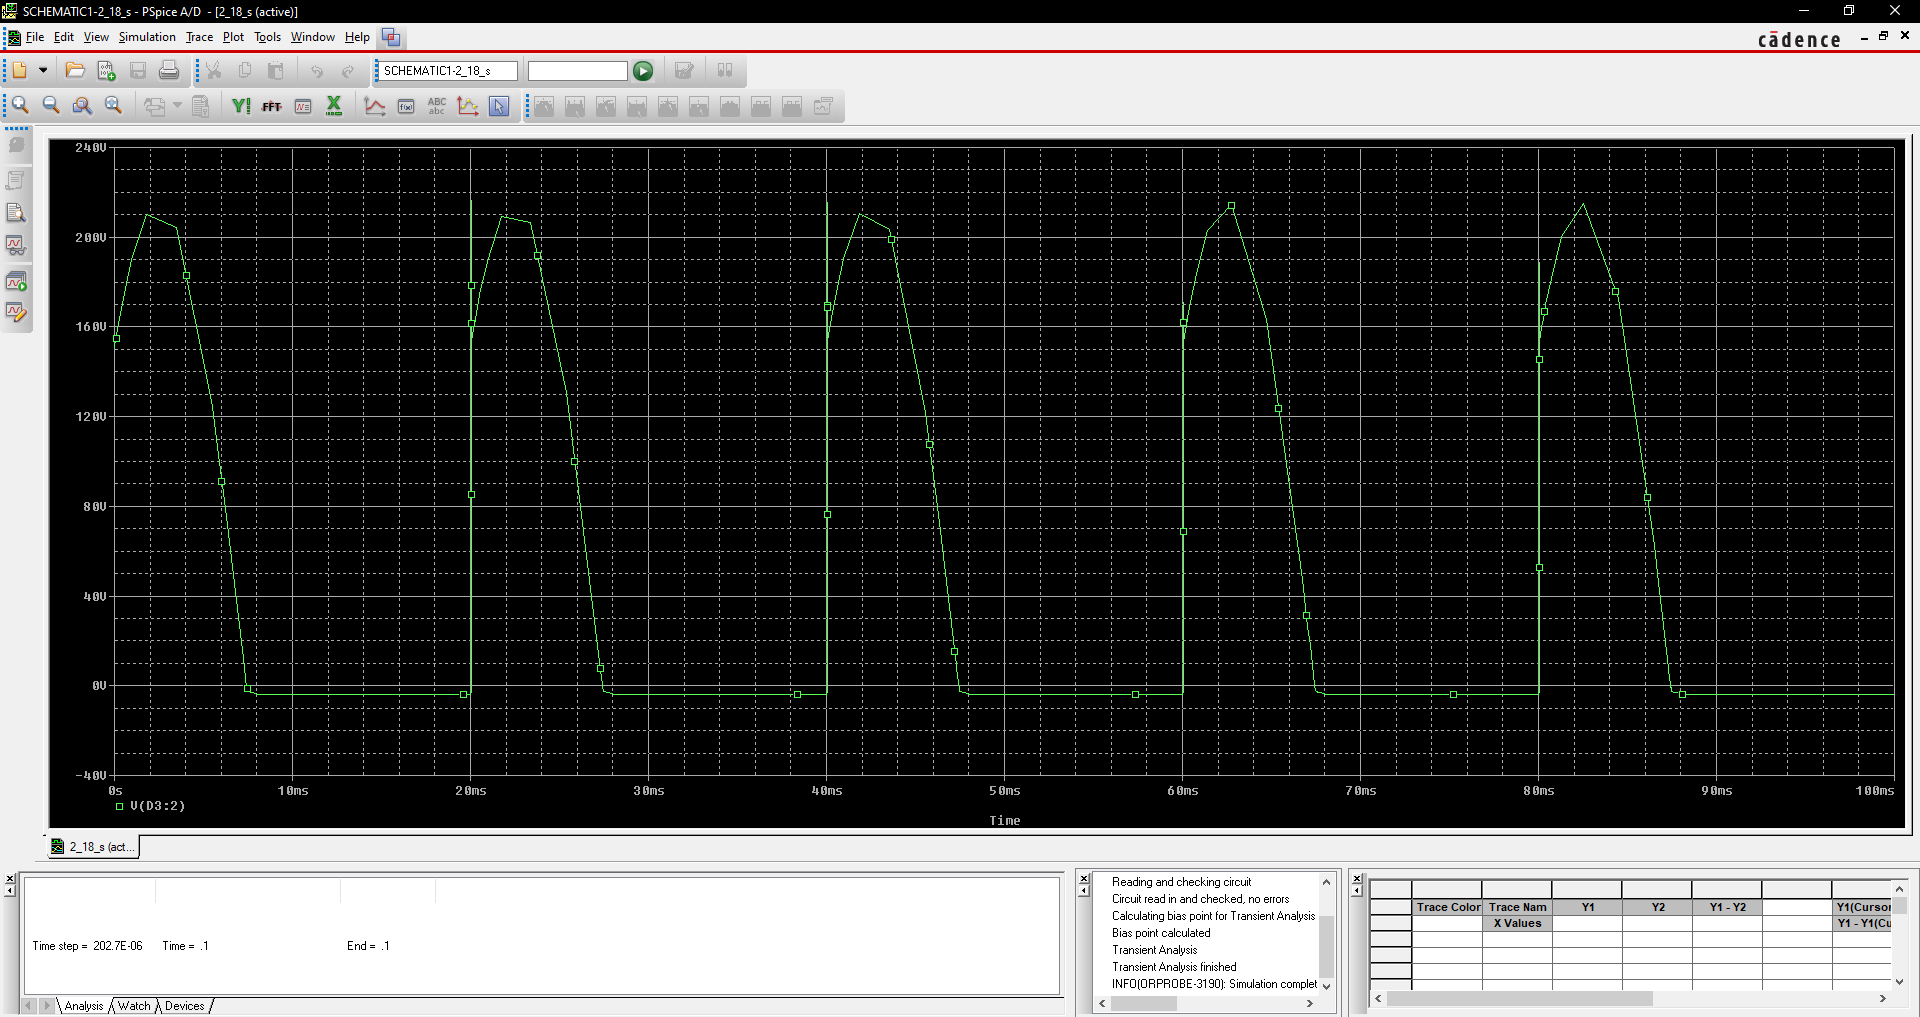
\includegraphics[width=13cm]{img/Sim/44.png}\\\\
    5.\\\\
    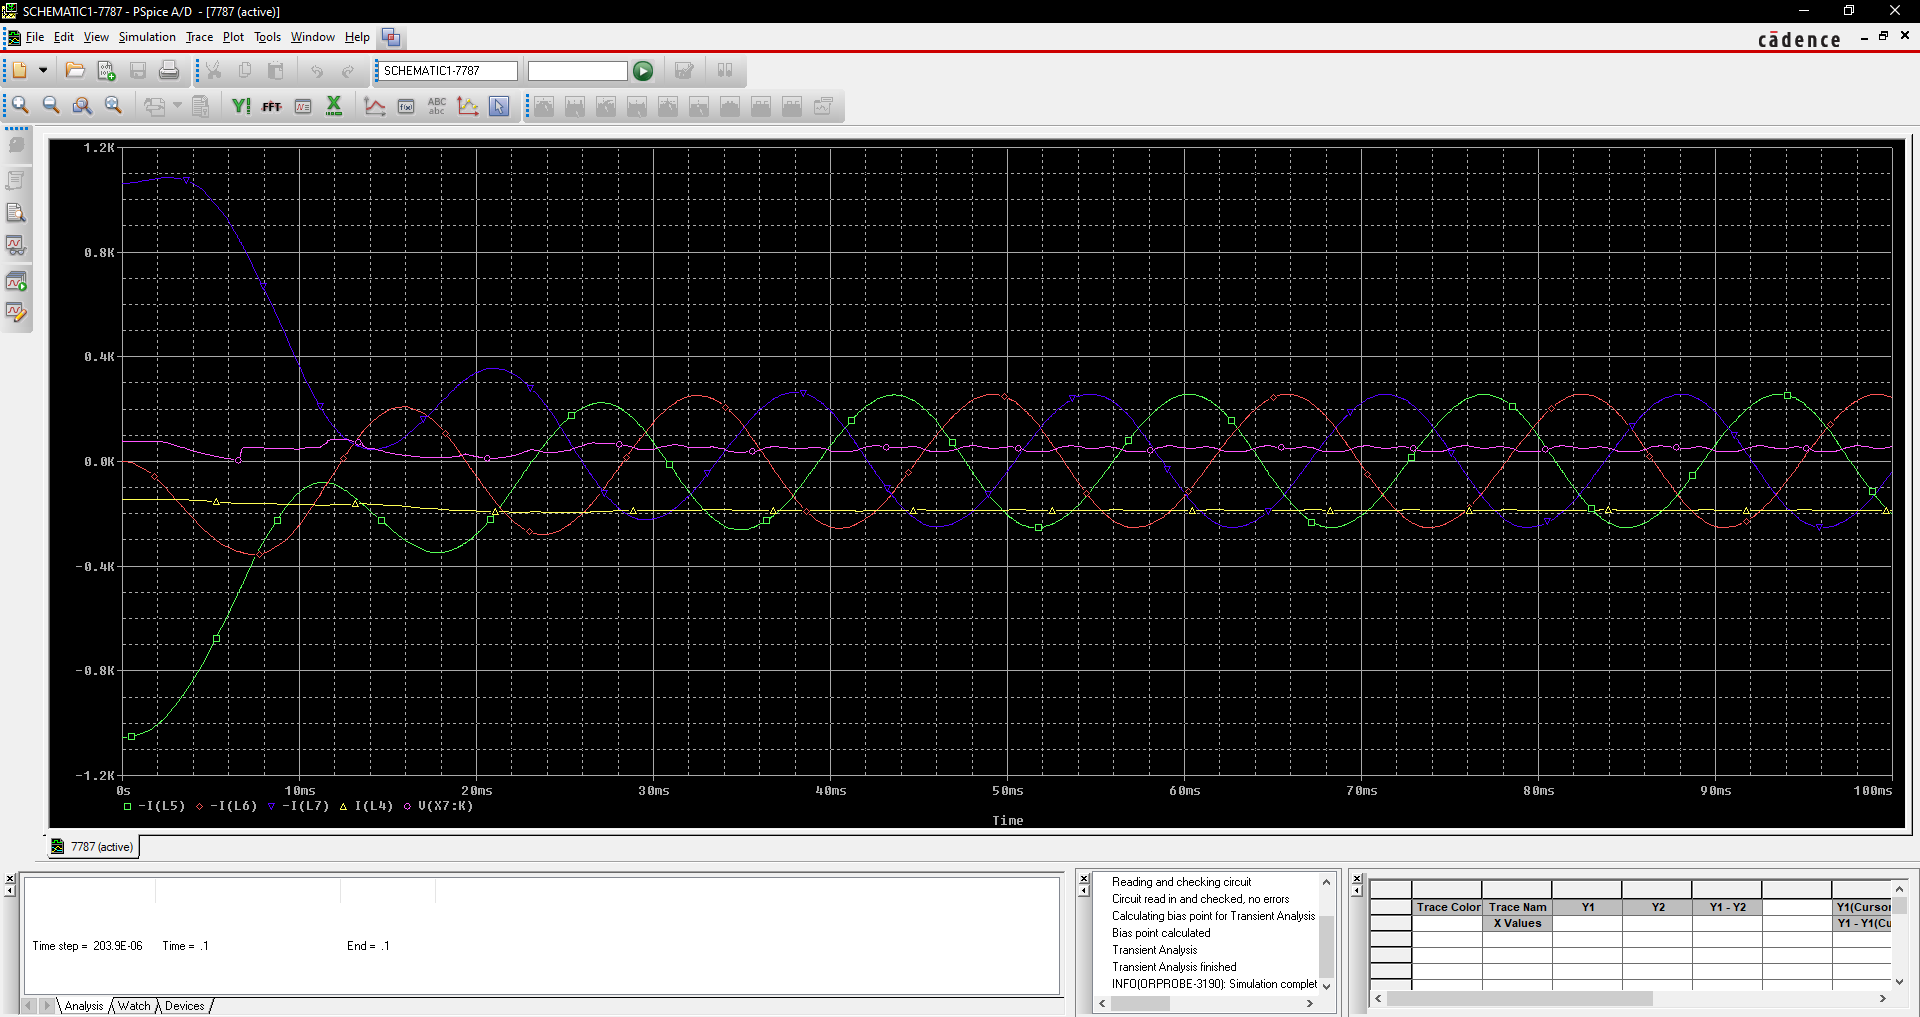
\includegraphics[width=13cm]{img/Sim/5.png}\\
    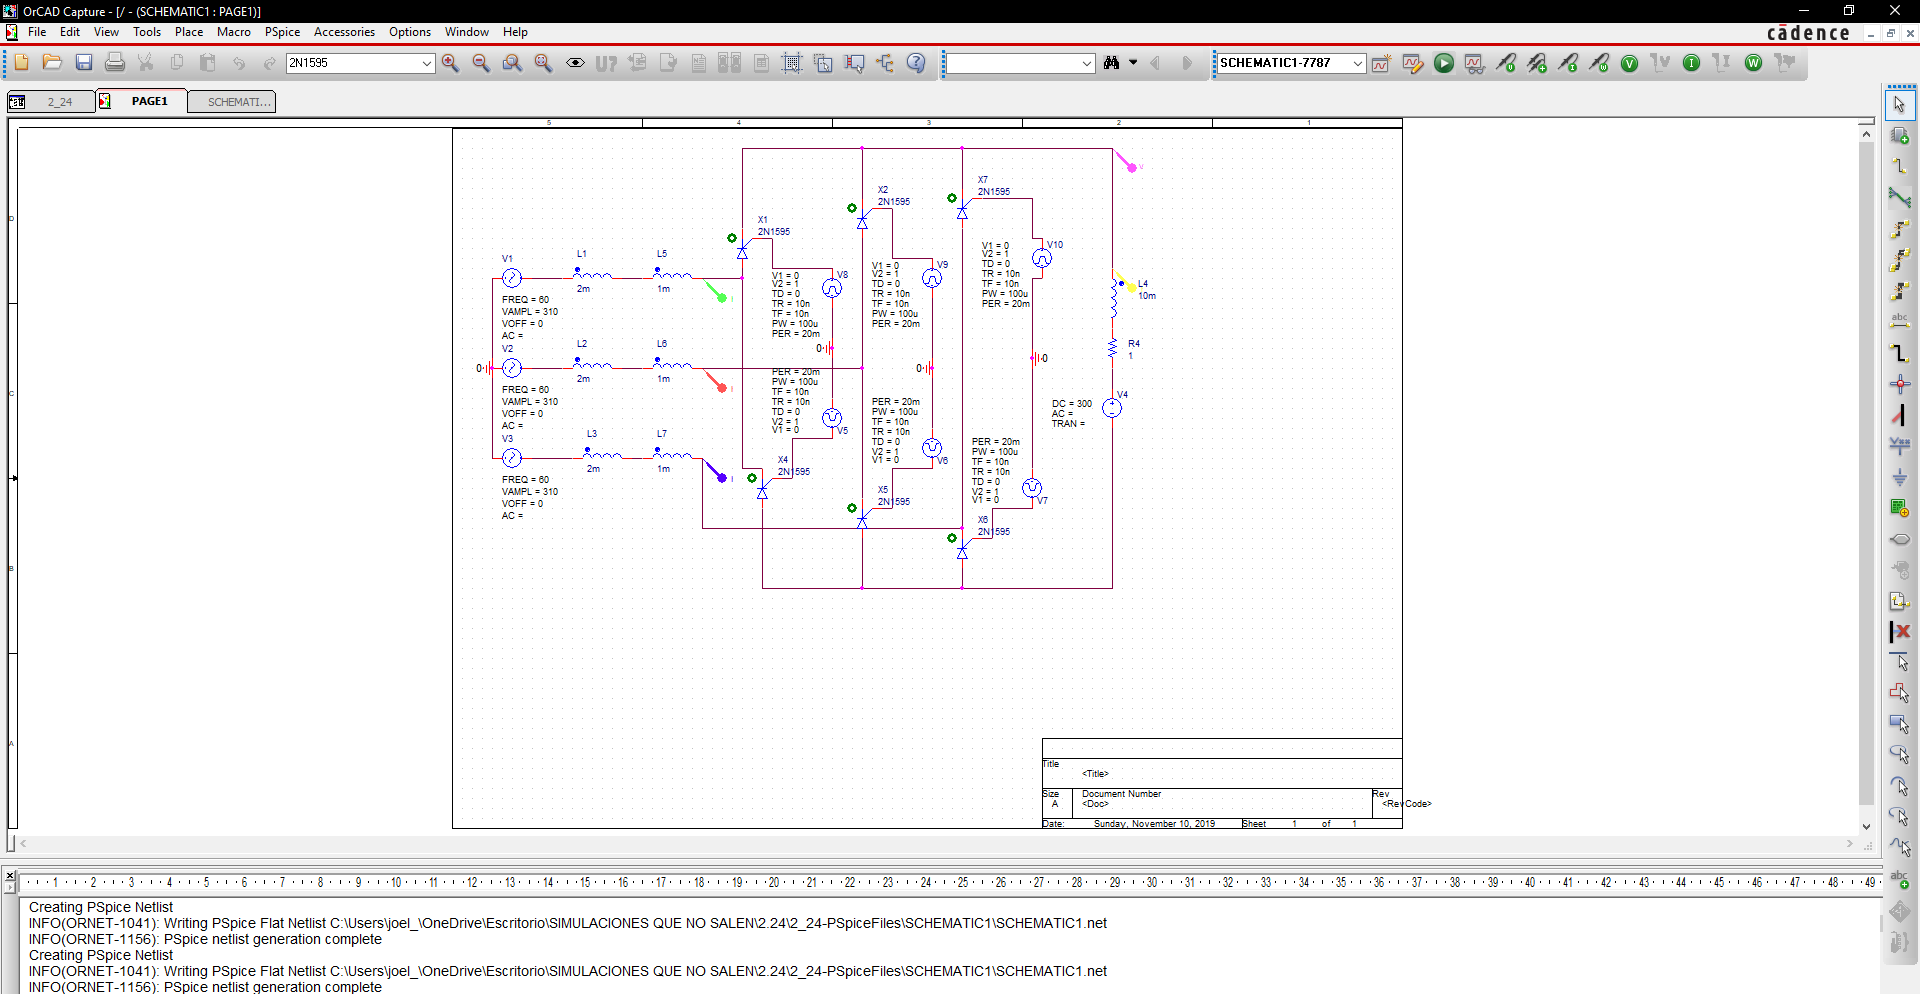
\includegraphics[width=13cm]{img/Sim/55.png}\\\\
    6.\\\\
    
\end{large}




   
    

\begin{LARGE}
\textbf{Conclusión:}\\
\end{LARGE}
\begin{large}
  1.-  El diac tiene un voltaje de activacion que le permite conducir la corriente a traves de el, y permitir la activacion del triac, en el caso de este diac son 30v.\\
    En este circuito el capacitor tiene una funcion muy importante que es almacenar el pulso requerido para que el diac conduca y el triac se active, es por eso que el capacitor es de baja capacitancia, para no modificar la señal de ninguna manera.\\
    Este circuito es util en la industria para la regulacion de las faces de una revolvedora, controlar intesidad de luz el algunos tratamientos haciendole los respectivos cambios.\\
2.- Mediante los tirirstores se puede hacer una regulación de voltaje importante en la corriente eléctrica que entra al circuito.\\
    La regulación realizada por el circuito depende mucho de los pulsos aplicados a los mismos.\\
\end{large}





\begin{LARGE}
\textbf{Bibliografía:}\\
\end{LARGE}
    URL: https://www.areatecnologia.com/electronica/tiristor.html\\
    Website Title: temas de tecnologia\\
    Access Day: 11\\
    Access Month: november\\
    Access Year: 2019\\
    Article Title: Tiristor\\






\end{document}
